\cleardoublepage
\chapter{The fastPSI protocol}
\label{chapter:protocol}

% \todo{
% Add an ``overview'' section with a figure that explains the protocol at a high level, step by step. We can do it as an example, denoting the messages between client and server. We can also say how the state (assuming an initial one) evolves with each step.

% Another option is to use this figure in two places. In overview, the figure will explain the messages and steps. In the detailed section, use the figure as a running example.

% Tradeoff of 2pc vs Saeida Ardekani et al. atomic multicast (the difference with NMSI)

% Design tradeoffs?
% }

In this chapter, we describe fastPSI, a transactional protocol that implements Parallel Snapshot Isolation while allowing stronger consistency guarantees for transactions accessing objects inside \emph{entity groups}. We begin with an overview of what entity groups are, and by explaining the consistency guarantees of fastPSI for transactions executing both within and across different entity groups. We follow with a summary of how the different participants of the protocol interact with each other, and with a description of the different data structures involved. Next, we show how the protocol is structured by going over the execution of a transaction. We conclude with a discussion of the possible drawbacks of the design.

\section{Consistency Guarantees}

The fastPSI protocol considers a system in which objects are aggregated in \emph{entity groups}~\citep{baker_megastore}. An entity group $\sigma$ is defined as a proper partition of objects $\Obj$. This means that two properties hold: (i) $\forall \sigma, \sigma' \implies \sigma \cap \sigma' = \emptyset$ and (ii) $\forall x \in \Obj .\ \exists \sigma .\ x \in \sigma$. The first property says that the sets of objects covered by different entity groups are \emph{disjoint}, while the second property states that any object that exists in the system is part of an entity group.

The goal of fastPSI is as follows: transactions that only access objects inside a single entity group should satisfy Snapshot Isolation (SI), while transactions that access objects across entity groups should satisfy Parallel Snapshot Isolation (PSI). Intuitively, if one has a single entity group that encompasses every object, any execution of fastPSI is equivalent to an execution under Snapshot Isolation. Conversely, if one has a entity group per object in the system, then any execution of fastPSI is equivalent to an execution under Parallel Snapshot Isolation. The decision of which objects to place into different entity groups is left to the programmer, who should take application requirements into account.

Recall from Section~\ref{sect:si} that transactions executing under SI are only partially ordered, in contrast with Serialisability, where they are totally ordered. However, the requirement for transactions to take monotonic \emph{start} and \emph{commit} timestamps induces a total \emph{commit order} for transactions, even for those that are not in conflict with each other. In the presence of different entity groups, this requirement would require transactions to communicate with every group in order to determine a monotonic timestamp. In fastPSI, we relax this requirement so that transactions have multiple, independent timestamps, one per each entity group.

In order to guarantee Parallel Snapshot Isolation across entity groups, we incorporate the notion of forward freshness~\citep{ardekani_nmsi}, which allows a transaction $\tx$ to read versions of objects written by transactions that committed after $\tx$ starts. Our protocol accomplishes this by making a transaction $\tx$ fix its start timestamp at a particular entity group only when $\tx$ reads an object from that group. This also allows a transaction to acquire start timestamps only at the groups it reads from, and avoids coordination with other groups.

Our protocol leverages both approaches to offer its consistency guarantees: a transaction is able to read from versions written by latter transactions as long as those reads form a \emph{causally consistent snapshot}. When a transaction $\tx$ performs its first read operation in an entity group, it fixes a snapshot that includes all the transactions that committed before $\tx$'s read occurred. As $\tx$ performs further read operations on other entity groups, the snapshots that $\tx$ fixes are restricted to versions written by transactions that are not causally dependent on the transactions that $\tx$ already included in its previous snapshots.

\section{Overview and System Model}

The protocol consists of three components: \emph{client} processes that provide the system interface for managing transactions, \emph{server} processes that handle the individual operations of transactions, and \emph{entity groups}---managed by a server---which store individual data objects. Given that entity groups properly divide the range of objects into disjoint \emph{partitions}, for the remainder of this chapter we use the term partition as a shorthand for entity group.

Both client and server processes are considered reliable and connected by reliable channels\footnote{Fault-tolerance concerns are orthogonal to the problem we address, but several approaches are discussed in Chapter~\ref{chapter:related_work}.}. Processes communicate with each other using an asynchronous message-passing system. We denote the server processes as a set $\mathcal{S} = \{s_1, \dots, s_N\}$, and clients as $\mathcal{C} = \{c_1, \dots, c_M\}$. Data objects are denoted by a set $\Obj$, split into $N$ partitions, each stored by a server process. We let $\partitionOf(x)$ be the index of the partition the object $x$ belongs to, so that it is managed by server $s_{\partitionOf(x)}$.

\emph{Clients} provide the transactional interface of our protocol through the \texttt{start}, \texttt{read}, \texttt{write} and \texttt{commit} operations. Transactions are \emph{interactive}, i.e., when a transaction starts, the client does not know which operations it will perform in advance. The fastPSI protocol uses optimistic concurrency control, and therefore the \texttt{start} and \texttt{write} operations are local to the client. Clients issue \texttt{read} operations to servers, which in turn communicate with its partitions and return the values and metadata associated with the objects the client requested. Clients handle \texttt{write} operations locally by storing the updates in a buffer. At \texttt{commit} time, the client acts a coordinator of a \emph{two-phase commit protocol (2PC)}~\citep{bernstein_concurrency} among all the participating servers, issuing \texttt{prepare} and \texttt{decide} operations. The written values buffered locally are transmitted to the servers at \texttt{prepare} time, together with the accumulated metadata for the objects that the client read. The decision to commit or abort a transaction is taken based on this metadata.

\emph{Servers} handle three operations issued by clients: \texttt{read}, \texttt{prepare} and \texttt{decide}. When a server handles \texttt{read} operations, it forwards the request to the partition responsible for the object being requested. When receiving a \texttt{prepare} request for a certain transaction, the server checks for conflicts with other transactions waiting to be decided, which are stored in a commit queue. If the transaction contained in the client request does not conflict, it is added to the queue, and the server replies to the client with a $\commit$ vote. If, on the other hand, the transaction is found to be conflicting, an $\abort$ vote is sent instead.

\emph{Partitions} are responsible for fulfilling read requests on behalf of servers, and for maintaining causally consistent snapshots on behalf of the clients. Partitions store multiple \emph{versions} of an object in accordance with a multi-version concurrency control protocol. When executing a read request for an object $x$, a partition finds and returns the most recent causally consistent version of $x$, along with some metadata of the chosen version.

Each partition stores multiple version of an object represented by a tuple $\langle val, vid \rangle$, where $val$ is the value of a given version, and $vid$ is a logical identifier for the transaction that committed this version. To represent this logical identifier we use \emph{version vectors}~\citep{version-vectors}. Such a vector consists of $N$ entries, one for each partition, storing a non-negative integer. Each entry $vid[i]$ in the vector can also be represented by a pair $(s_i, k)$, where $k$ is the actual value of the $i$-th entry of the vector. We call these pairs a dot~\citep{carlos-causality}. Version vectors are compared according to the following relation, showing when one vector covers more dots than another: $V_1 \sqsubseteq V_2 \iff \forall i.\ V_1[i] \le V_2[i]$. In addition, there exists a \emph{join} operation on vectors, taking their entry-wise maximum.
% We will denote this operation by $\max$ from now on.
We also denote the set of all version vectors by $\VCSet$, and the vector with all entries set to $0$ by $\vec{0}$.

\section{Server data structures}

\begin{figure}[t]
\noindent\adjustbox{max width=\paperwidth}{\footnotesize
\begin{tabularx}{\linewidth}{|c|p{5.5cm}|X|}
  \hline
  \multicolumn{3}{|c|}{\textbf{Variables at a server $s_i$}}\\
  \hline
  $\lastprep$ & {\sf Integer} & The number of update transactions that tried to
  commit at the server.
\\
  \hline
  $\VersionLog$ & ${\sf Map}[\keytype,$ ${\sf
    Set}[\langle \valuetype\ \val, \vctype\ \Vcomm\rangle]]$ & Database:
  a mapping from objects to lists of pairs of a value and the
  commit vector of the transaction that wrote it. The lists are ordered
  by the $i$-th component of the commit vectors.
\\
  \hline
  $\CommitLog$
  & ${\sf Sequence}[\langle\transtype\ T,$ $\vctype\ \Vaggr \rangle]$
  & Log of update transactions $T$ committed at the server, ordered by
  $\Vaggr[i]$. Here $\Vaggr$ is the aggregate vector of $T$: the join of the
  commit vectors of all transactions up to $T$ in $\CommitLog$.
\\
  \hline
  $\LocalTime$ & $\vctype$ & The join of the commit vectors of all
  transactions in $\CommitLog$.
\\
  \hline
  $\CommitQueue$ & ${\sf Sequence}[\langle \transtype, \pending, {\sf WriteSet} \rangle \cup
  \langle \transtype, \ready, {\sf WriteSet}, \vctype\rangle]$ &
  Queue containing information about update transactions trying to commit
  at the server.
\\
  \hline
  \hline
  \multicolumn{3}{|c|}{\textbf{Context for a transaction $T$ at a client $c_i$}} \\
  \hline
  $T.\WS$ & ${\sf WriteSet}$ & Write-set of $T$.
\\
  \hline
  $T.\hasRead$ & ${\sf Vector}[{\sf Bool}]$ & Mapping showing whether $T$  has
  read a given partition.
\\
  \hline
  $T.\VCaggr$ & $\vctype$ & Snapshot vector: determines snapshots fixed at
  partitions $T$ has read from and possible causal dependencies at all other
  partitions.
\\
  \hline
  $T.\VCdep$ & $\vctype$ & Dependency vector, representing all causal
  dependencies developed by $T$ during its execution.
\\
  \hline
\end{tabularx}
}
\caption{List of variables used in the protocol, where
  ${\sf WriteSet} = {\sf Set}[\langle \keytype, \valuetype \rangle]$. The orders
  of entries in $\CommitLog$, $\VersionLog$ and $\CommitQueue$ are consistent
  with the commit order of transactions the entries are associated with. We
  select the components of various tuples using the names given in the figure.}
\label{fig:prot-ds-table}
\end{figure}

Each server $s_i$ maintains five main data structures: $\lastprep$, $\VersionLog$, $\CommitLog$, $\LocalTime$ and $\CommitQueue$. Their role is summarised in Figure~\ref{fig:prot-ds-table}. We follow with a more detailed explanation of each of them.

$\lastprep$ is a counter of the number of update transactions that initiated their commit phase at a given server. When a transaction commits at a server $s_i$, it is assigned a \emph{sequence number} $k$ derived from this counter. This sequence number induces the \emph{commit order} of transactions at $s_i$. A transaction computes its \emph{commit vector} $V_c$ from these sequence numbers, such that the vector represents the set of dots $\{(s_i, k) \mid k \le V_c[i]\}$, which identifies the writes by previous transactions whose sequence number at a server $s_i$ is no higher than $V_c[i]$.

$\VersionLog$ is a mapping of objects to a list of versions, which we call the \emph{database}. As noted before, each version is a tuple $\langle \mathsf{val},\ \Vcomm \rangle$ such that $\mathsf{val}$ is a value and $\Vcomm$ is the commit vector of the transaction that wrote $\mathsf{val}$. The $\VersionLog$ at $s_i$ is ordered by the $i$-th component of the commit vector of each version, which follows the commit order of transactions at the server. We denote by $\VersionLog[x].\last$ the most recent entry in the list for the object $x$.

$\CommitLog$ is an ordered list that maintains, for each update transaction that committed at a server, the tuple $\langle T,\ \Vaggr \rangle$, such that $\tx$ is the identifier of a committed transaction and $\Vaggr$ is an \emph{aggregate vector}. The aggregate vector represents the join of the commit vectors of all the transactions up to $\tx$ in $\CommitLog$. Entries in the log at $s_i$ are totally ordered according to the $i$-th entry of their aggregate vectors, $\Vaggr[i]$, which also follows the commit order of transactions at the server. These aggregate vectors are stored for efficiency, and are used to compute the snapshot of a transaction at the server. The aggregate vector of the last committed transaction is stored in $\LocalTime$. Initially, the $\CommitLog$ contains a single placeholder entry $\langle \_, \vec{0} \rangle$.

Finally, $\CommitQueue$ is an ordered queue of transactions trying to commit updates at the server. The queue has entries of two types. An entry $\langle \pending, \tx, \localWS \rangle$ means that $\tx$ is successfully prepared to commit at $s_i$, but the final decision on it is not yet known; $\localWS$ is the \emph{write-set} of the transaction, containing object-value pairs. An entry $\langle \ready, \tx, \localWS, V \rangle$ in the queue means that $\tx$ has been decided to commit with a commit vector $V$, but its writes have not yet been added to the $\VersionLog$. The order of transactions in $\CommitQueue$ follows the commit order at the server.

\section{Protocol Description}

We now describe in detail how the protocol works by following the execution of a transaction. We begin by describing how a transaction is initialised, along with the mechanism to build a causally consistent snapshot. Later, we show the mechanism to validate and commit a transaction.

\subsection{Transaction Execution}

\begin{figure}[h]
\begin{algorithm}[H]
  \setcounter{AlgoLine}{0}
  % Start
  \SubAlgo{\Fun ${\tt start}()$\label{alg:start_tx_start}}{
    \Return{$\KwSty{new}\ \transtype(\WS= \emptyset, \hasRead =
      \vec{\bot}, \VCaggr = \vec{0}, \VCdep =
      \vec{0})$};\label{alg:start_tx_end}}

  \smallskip

  % Write
  \SubAlgo{\Fun ${\tt write}(T, x, v)$\label{alg:write_start}}{
    $\tx.\WS \leftarrow \left(\tx.\WS\ \backslash\ \{\langle x, \_ \rangle\}\right) \cup \{\langle x,v\rangle\}$\;\label{alg:write_end}
  }
\end{algorithm}
\caption{Initialisation of a transaction and update of an object \emph{x} at client $c_i$.}
\end{figure}

A client executing a transaction $\tx$ maintains a transaction \emph{context} including several pieces of data, summarised in Figure~\ref{fig:prot-ds-table} and explained below. This context is initialised by the client when it starts a transaction (line~\ref{alg:start_tx_start}).

Since our protocol uses optimistic concurrency control, the execution of $\tx$ is speculative: clients read objects from servers and buffer writes locally. At the end of the execution, the decision whether to commit or abort a transaction is taken based on the existence of conflicts with concurrently executing transactions. When a transaction $\tx$ writes a value $v$ to an object $x$ (line~\ref{alg:write_start}), the client buffers this write in $\tx$'s \emph{write-set}, $\tx.\WS$, while discarding any previously written value of $x$.

When the transaction $\tx$ issues a read operation on an object $x$ (line~\ref{alg:read_start}), the client first checks $\tx.\WS$ (line~\ref{alg:read_ws_check}): if $\tx$ has already written to $x$, the value stored in the write-set is returned. Otherwise, and assuming that $j = \partitionOf(x)$, the client sends a $\READREQUEST$ message to the server $s_j$ to fetch the value of the object (line~\ref{alg:read_send}).

When the transaction $\tx$ reads an object from a partition $j$ for the first time, the server $s_j$ fixes a \emph{snapshot} of versions from which it will serve all future reads by $\tx$. This snapshot is defined by an integer $k$: it will include the versions written by all the transactions that committed at the server with a sequence number up to $k$. The client keeps this information in the transaction context, by storing $k$ in the $j$-th entry of a \emph{snapshot vector} $\tx.\VCaggr$, and by marking the current partition as read in $\tx.\hasRead$, a boolean mapping its $j$-th entry to $\top$ if $\tx$ read an object from $j$, and $\bot$ otherwise. If $\tx.\hasRead[j]=\top$, then the vector $\tx.\VCaggr$ is equal to the join of the commit vectors of all transactions that at partition $j$ have a sequence number no higher than $\VCaggr[j]$.

\begin{figure}[h]
\begin{algorithm}[H]
  % Read
  \SubAlgo{\Fun ${\tt read}(T, x)$\label{alg:read_start}}{
    \If{$\langle x, v \rangle \in \tx.\WS$\label{alg:read_ws_check}}{
      \Return{$v$}\;
    }

    $j \leftarrow \partitionof(x)$\;
    \Send{$\READREQUEST(x, T.\VCaggr, T.\hasRead)$} \KwTo $s_j$\;\label{alg:read_send}
    \Receive{$\READRETURN(m)$} \KwFrom $s_j$\;\label{alg:read_recv}
    \uIf{$m = \abort$} {
      \Throw{$\abort$}\;\label{alg:read_abort}
    }
    \ElseIf{$m = \langle v,\localVdep,\localVaggr \rangle$\label{alg:read_msg_decomp}}{
      $\tx.\hasRead[j] \leftarrow \true$\;
      $\tx.\VCdep \leftarrow \max(\tx.\VCdep,\localVdep)$\;\label{alg:read_upd_vcdep}
      $\tx.\VCaggr \leftarrow \max(\tx.\VCaggr,\localVaggr)$\;\label{alg:read_upd_vcaggr}
      \Return{$v$}\;\label{alg:read_end}
    }
  }

  \smallskip

  % ReadRequest
  \SubAlgo{\WhenReceived $\READREQUEST(x, \argVCaggr, \argHasRead)$ \KwFrom $c_j$\label{alg:read_req_start}}{
    \uIf{$\argHasRead[i]$\label{alg:read_req_read_check}} {
      $V \leftarrow \argVCaggr$\;\label{alg:read_req_read_maxvc}
    }
    \Else{\label{alg:read_req_read_check_else}
      \Until{$\mrvc[i] \ge \argVCaggr[i]$}\;\label{alg:read_req_wait}
      $r \leftarrow \max\{r \in \CommitLog \mid \forall j.\, \argHasRead[j] {\implies} \left(r.\Vaggr[j] \le \argVCaggr[j]\right)\}$\;\label{alg:max_vc_search}
      \If{$r.\Vaggr[i] < \argVCaggr[i]$\label{alg:read_req_abort_check}}{
        \Send{$\READRETURN(\abort)$} \KwTo $c_j$\;\label{alg:read_req_abort}
        \Return\;
      }
      $V \leftarrow r.\Vaggr$\;\label{alg:read_req_unread_maxvc}
    }
    $\ver = \max\{\ver \in \VersionLog \mid ver.\Vcomm[i] \le V[i]\}$\; \label{alg:chose-version}
    \Send{$\READRETURN(\ver.\val, \ver.\Vcomm,V)$} \KwTo $c_j$\;\label{alg:read_req_end}
  }
\end{algorithm}
\caption{Local and remote read of object \emph{x}.}
\end{figure}

Thus, the entries of the snapshot vector for partitions that $\tx$ has not yet read from delimit all the possible causal dependencies $\tx$ may develop at these partitions if it keeps reading objects from the snapshots it has already fixed.

Both $\tx.\VCaggr$ and $\tx.\hasRead$ are supplied by the client when issuing a read operation on object $x$, by using them as parameters to the $\READREQUEST$ message sent to a server $s_i$. When the server receives this message (line~\ref{alg:read_req_start}), it first checks, using the $\hasRead$ mapping, if the transaction has read from it before (line~\ref{alg:read_req_read_check}). In this case, the snapshot is determined by $\VCaggr[i]$, and the server returns the latest version $\mathit{ver}$ of the object $x$ written by a transaction in the snapshot, i.e., with a sequence number no higher than $\VCaggr[i]$ (line~\ref{alg:chose-version}). This version is determined by examining the $i$-th entry of the commit vectors in $\VersionLog$. The server then replies to the client with a $\READRETURN$ message containing the value of the chosen version and its associated version vector, as well as the unmodified snapshot vector provided by the client: since the server used a previously fixed snapshot, no updates to the vector are required.

% \begin{figure}[t]
% 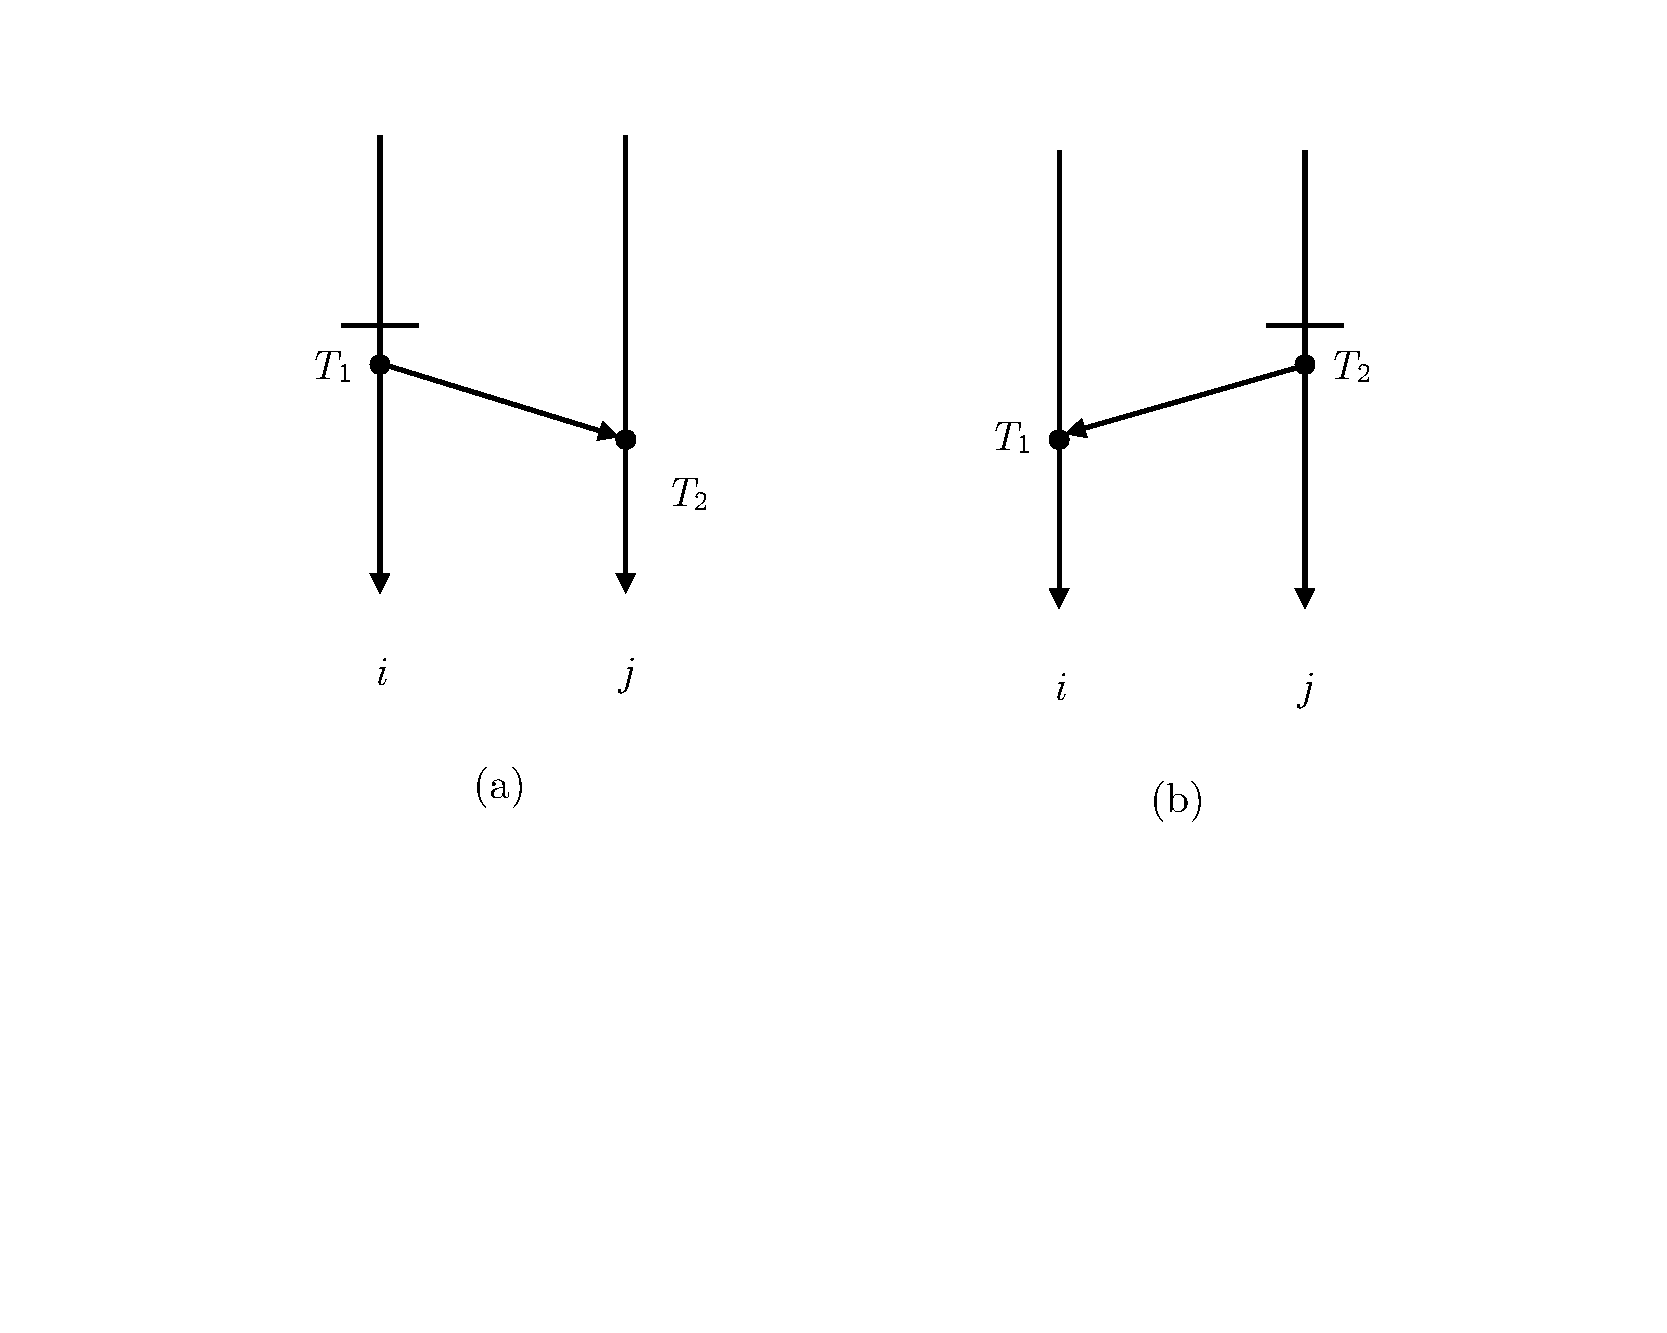
\includegraphics[width=\textwidth]{figures/ch4_snapshot_fork.pdf}
% \vspace{-5.5cm}
% \caption{Illustrations of the snapshot computation. Vertical lines depict the
%   commit order at the corresponding partitions (top to bottom) and horizontal
%   lines the cut-offs of various snapshots. Arrows between partitions depict
%   causal dependencies.}
% \label{fig:fig:snapshot_fork}
% \end{figure}

We now consider the case when the client is reading from the server $s_i$ for the first time (line~\ref{alg:read_req_read_check_else}), in which case, we have to fix the snapshot for the transaction $\tx$ at this server. Choosing a suitable snapshot is complicated by the fact that we allow transactions to be interactive---that is, we do not know in advance which objects will read in the future. We hence fix the snapshot in such a way that \emph{any} later read from this snapshot will be \emph{causally consistent} with any reads (past or future) from the snapshots that $\tx$ has already read, as specified by $\hasRead$ and $\VCaggr$. To ensure this, the snapshot we select has to satisfy two requirements.

\begin{figure}[t]
\vspace{-0.5cm}
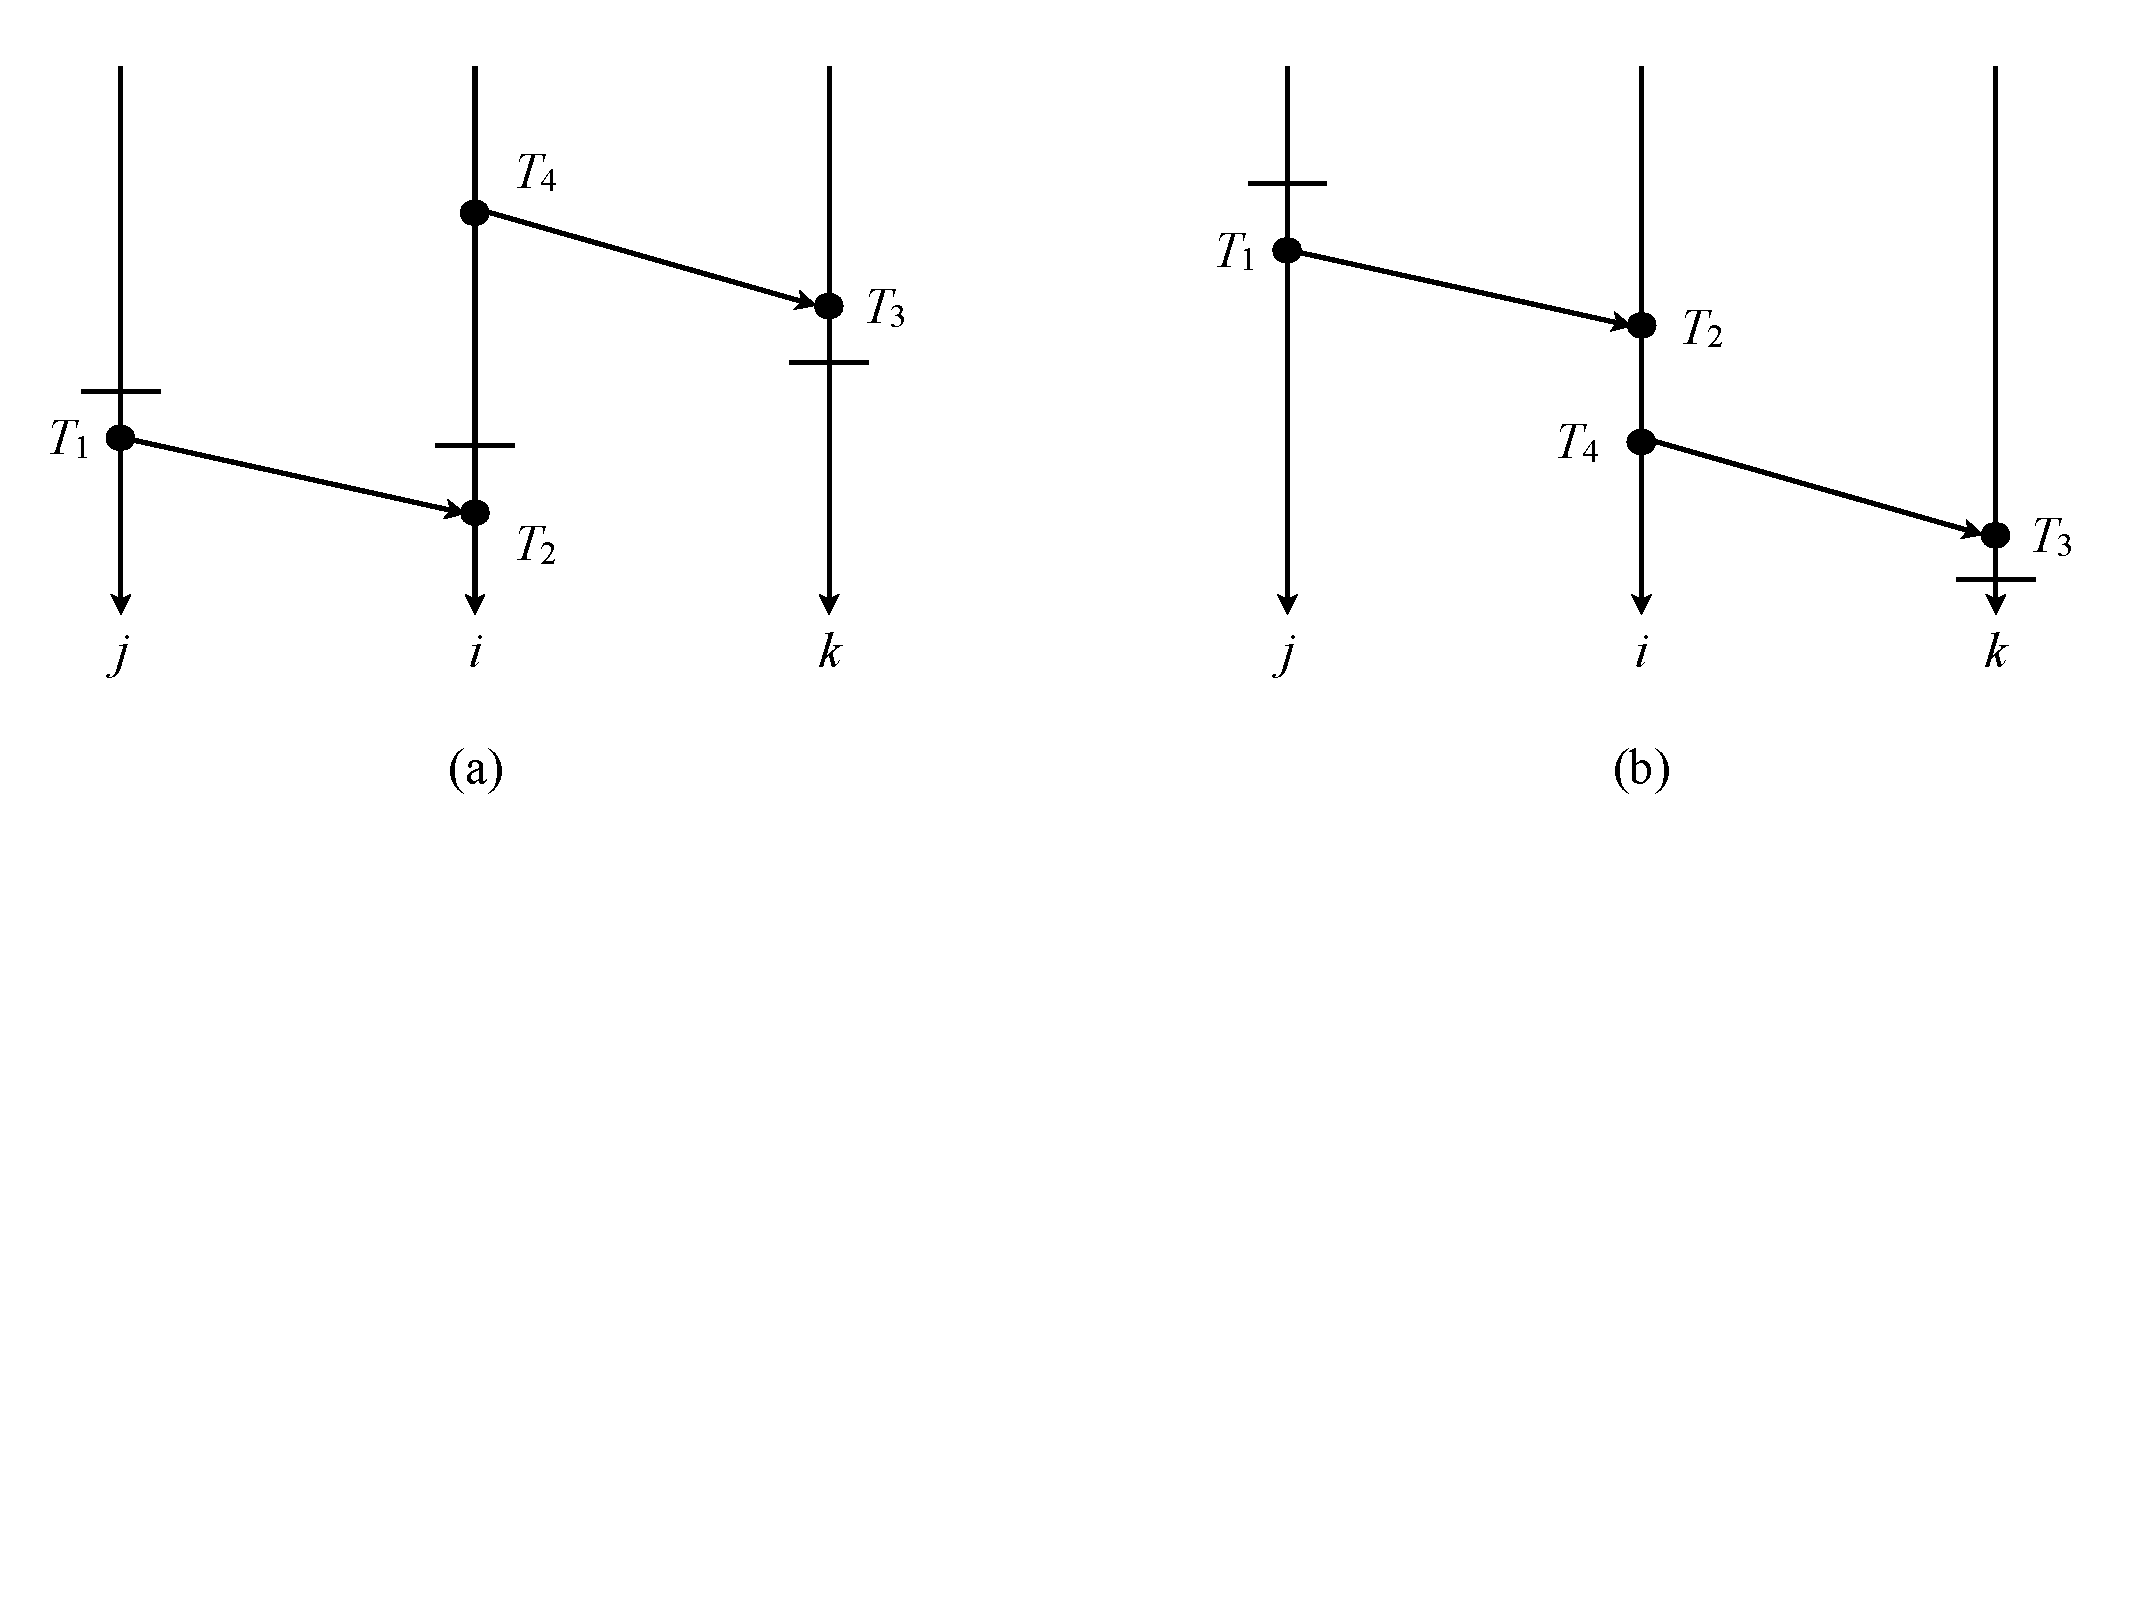
\includegraphics[width=\textwidth]{figures/ch4_snapshot.pdf}
\vspace{-6.5cm}
\caption{Illustrations of the snapshot computation. Vertical lines depict the
  commit order at the corresponding partitions (top to bottom) and horizontal
  lines the cut-offs of various snapshots. Arrows between partitions depict
  causal dependencies.}
\label{fig:snapshot}
\end{figure}

On the one hand, the snapshot cannot be too fresh. For example, suppose a transaction $\tx_1$ writing to some partition $j$ is excluded from the snapshot chosen by $\tx$ at $j$. Then, the snapshot chosen by $\tx$ at $i$ cannot contain $\tx_1$, nor any other transaction that causally depends on it, like $\tx_2$ (Figure~\ref{fig:snapshot}a). If the snapshot chosen by $\tx$ included $\tx_2$, it would be able to read some of $\tx_2$'s writes at $i$, thereby forcing $\tx$ to read the writes by $\tx_2$'s causal dependencies, including $\tx_1$; but $\tx$ cannot see these writes, because it excluded them from the snapshot at partition $j$. Thus, when building the snapshot, the server needs to take into account the snapshots taken by $\tx$ at the partitions it already read; the server selects the longest prefix of $\CommitLog$ transactions, such that their writes---and the ones by their causal dependencies---are included in $\tx$'s previous snapshots. This prefix is denoted by $r$ (line~\ref{alg:max_vc_search}), and is computed using the $\Vaggr$ vector included in each of the entries of $\CommitLog$, summarising the causal dependencies of all transactions up to a given record in the log. Thus, the snapshot at $s_i$ includes all transactions with sequence numbers up to $r.\Vaggr[i]$.

On the other hand, the snapshot selected cannot be too stale. Continuing with the previous example, if a transaction $\tx_3$ is included in the snapshot taken by $\tx$ at some partition $k$, then the snapshot of $\tx$ at partition $i$ has to include the writes by $\tx_3$ and its causal dependencies, e.g., the transaction $\tx_4$ in Figure~\ref{fig:snapshot}a. The writes of transactions---and of its causal dependencies---in the snapshots that $\tx$ has already fixed are summarised by $\VCaggr$. Thus, after determining the appropriate snapshot in line~\ref{alg:max_vc_search}, the server $s_i$ checks that this snapshot covers transactions with sequence numbers at $i$ up to $\VCaggr[i]$ (line~\ref{alg:read_req_abort_check}). To maximise the chances of passing this check, before allowing a transaction $\tx$ to proceed with a read, the server $s_i$ waits until the writes from the prefix up to $\VCaggr[i]$ have been incorporated into its state (line~\ref{alg:read_req_wait}).

It may be the case that it's impossible to satisfy both of the above requirements when selecting a snapshot; e.g., in the situation illustrated in figure~\ref{fig:snapshot}b. Assuming that the transaction $\tx$ has fixed a valid snapshot at $j$ and $k$, it is impossible to build a consistent snapshot at partition $i$; given that $\tx$ included $\tx_3$ at partition $k$, it is forced to read $\tx_4$'s writes at $i$. At the same time, because it excluded $\tx_1$ from the snapshot at $j$, $\tx$ can't read the writes by $\tx_2$ at $i$. In this case, without our second requirement, the server $s_i$ would build a snapshot excluding both $\tx_2$ and $\tx_4$, violating $T$'s causal dependency on $\tx_3$. In this case the server sends to the client a $\READRETURN$ message with a special value $\abort$ (line~\ref{alg:read_req_abort}), which will cause the client to abort the transaction (line~\ref{alg:read_abort}).

Once the server fixes a new snapshot, it selects the most recent version of the object $x$, defined by $e.\Vaggr[i]$ (line~\ref{alg:chose-version}), to return to the client. The server replies with a $\READRETURN$ message, carrying a triple of the value of the object, its associated version vector, and the aggregate vector for $e.\Vaggr$, summarising the causal dependencies of all the transactions in the snapshot. When the client receives the message (line~\ref{alg:read_msg_decomp}), it first sets the $j$-th entry of $\tx.\hasRead$ to $\top$, to indicate that $\tx$ has read an object at partition $j$, and joins the returned aggregate vector to $\tx.\VCaggr$. The client also joins the commit vector associated with the version read to a \emph{dependency vector} $\tx.\VCdep$, which represents all causal dependencies developed by $\tx$ during its execution. This ensures that, upon reading a version of object $x$, $\tx$ will causally depend on the transaction $\tx'$ that wrote that version of $x$, along with the causal dependencies of $\tx'$.

\begin{figure}[t]
\vspace{-2cm}
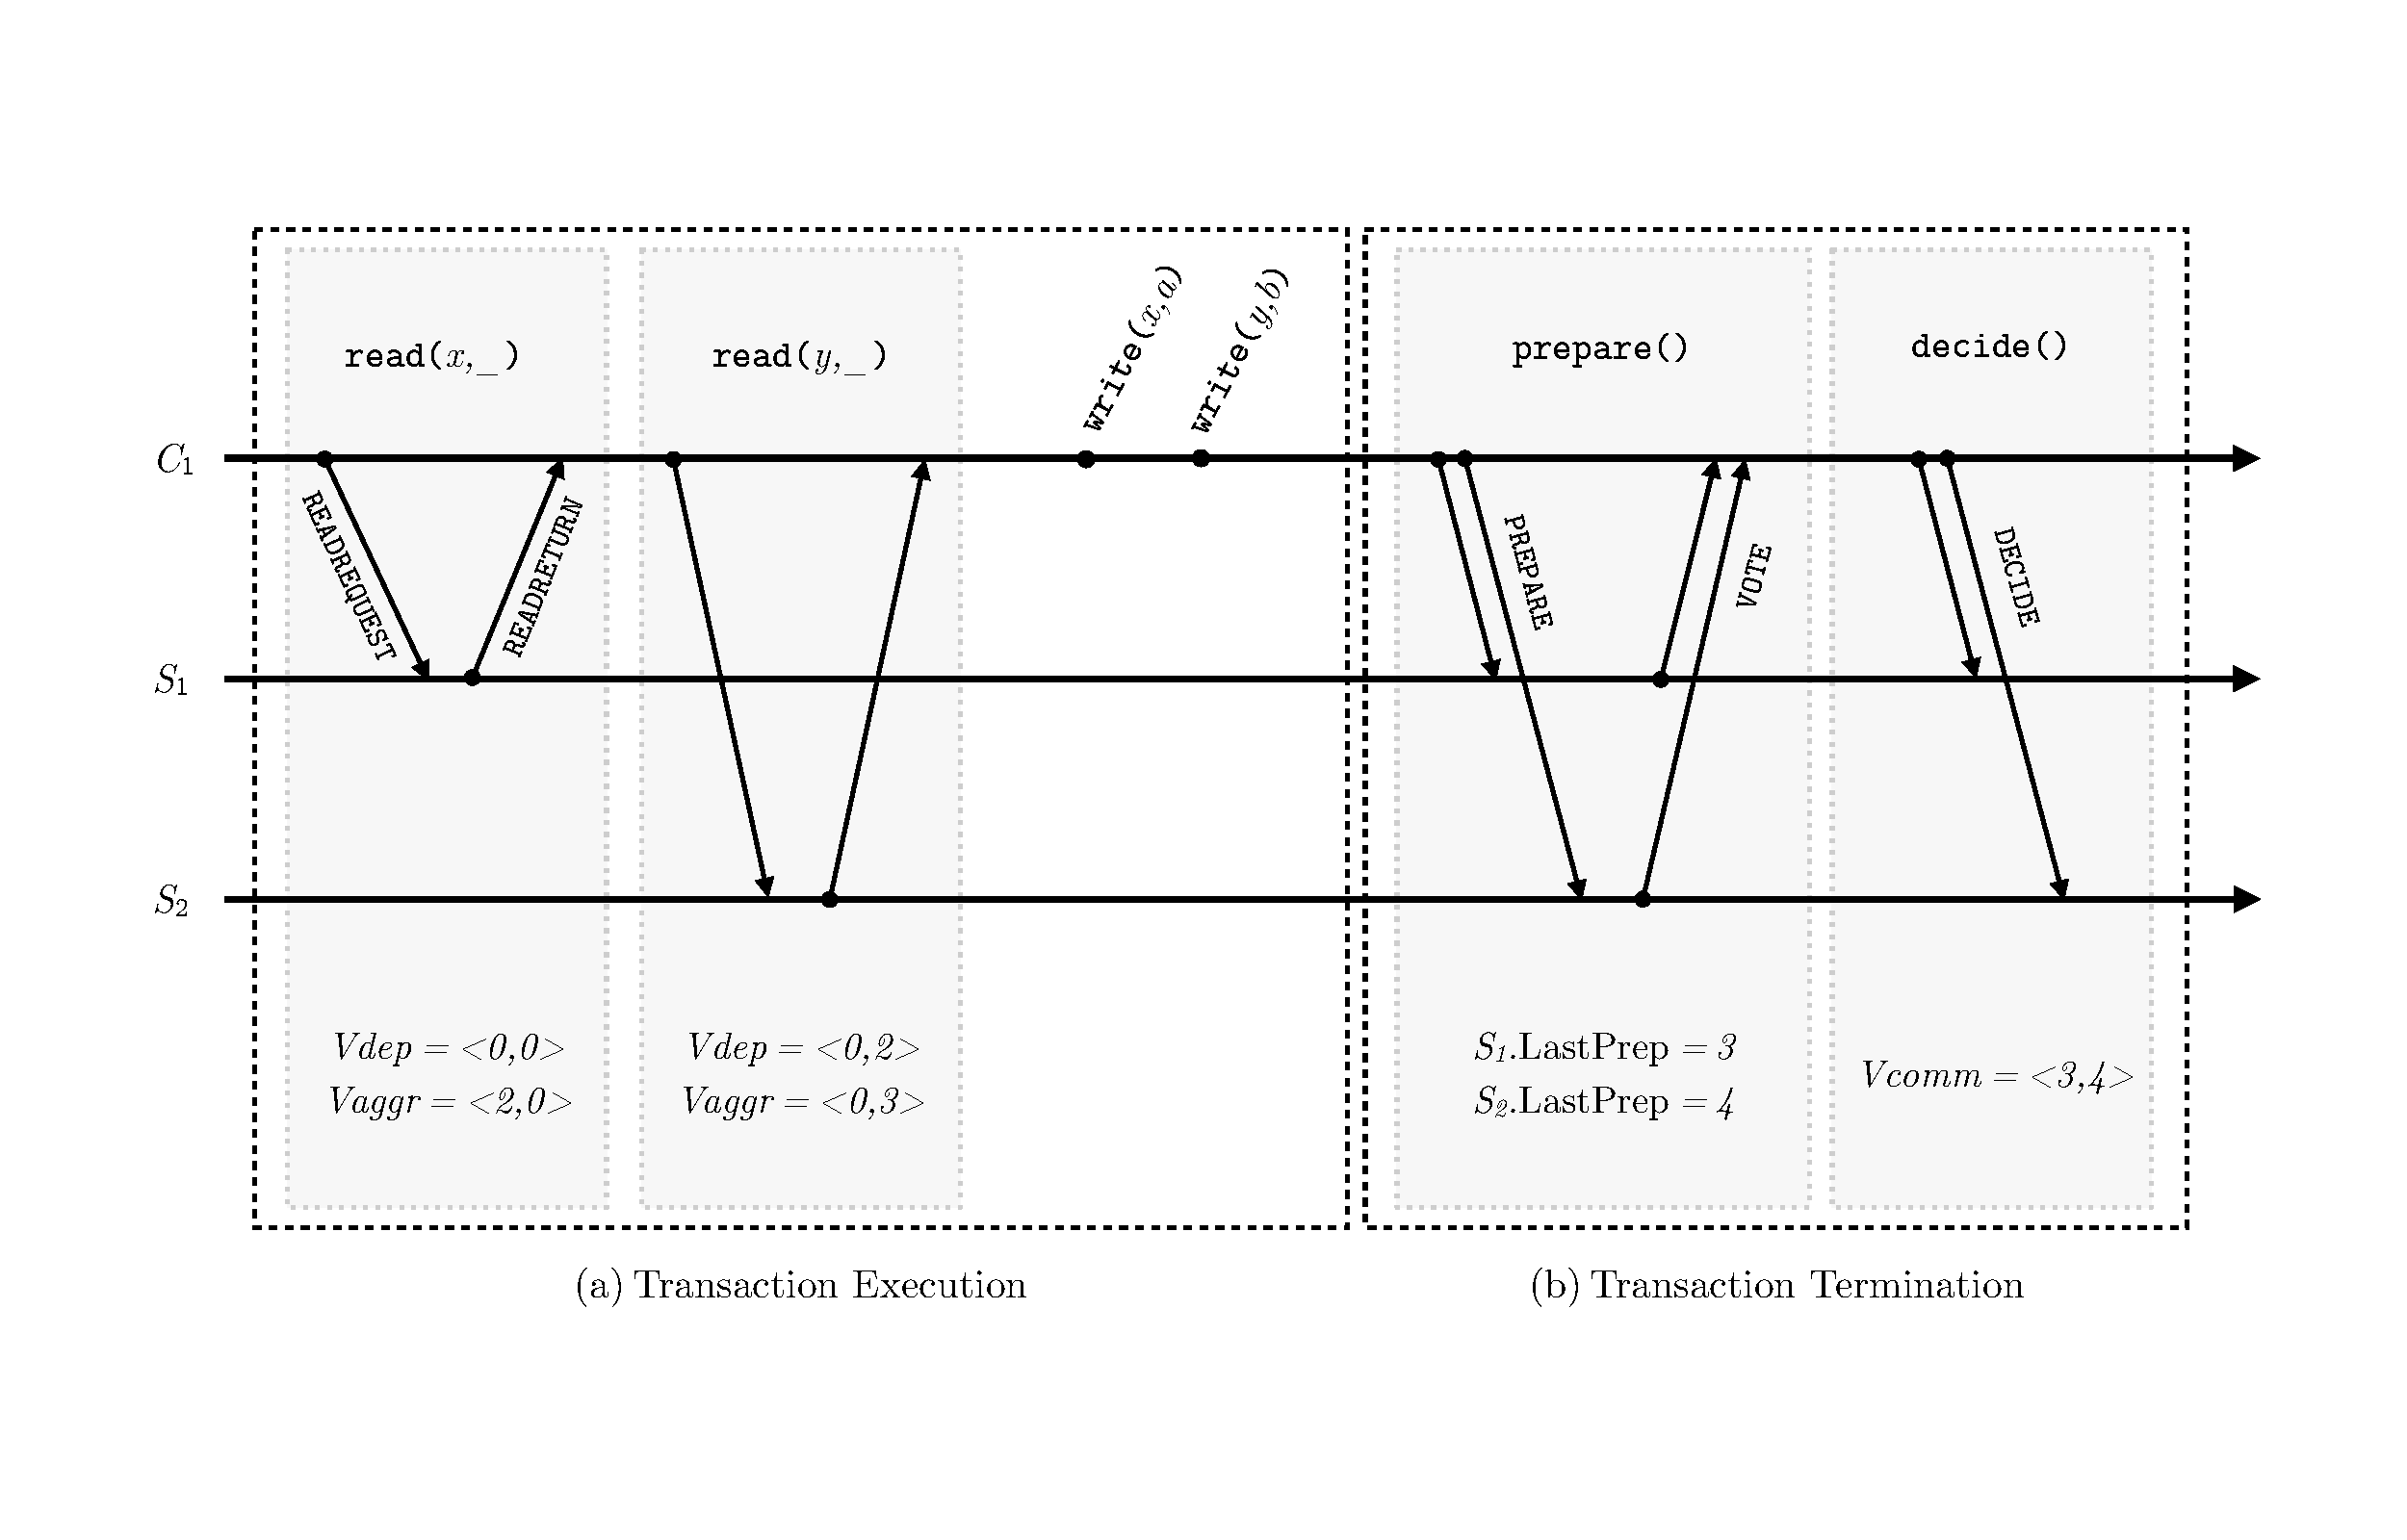
\includegraphics[width=\textwidth]{figures/ch4_execution.pdf}
\vspace{-2cm}
\caption{Message flow diagram of a sample execution, with message arrows labeled with their names in the protocol. The different interactions between a client and servers are shown in the shadowed regions. The operation performed by the client is shown at the top, and the state observed by the client at the end of each message exchange is summarised at the bottom.}
\label{fig:sample_execution}
\end{figure}

Consider the example depicted in Figure~\ref{fig:sample_execution}a. Client $c_1$ issues a pair of read requests to servers $s_1$ and $s_2$. In turn, these servers reply with the value of the object requested, along with its version vector and the new aggregate vector for the transaction, denoted by $\VCdep$ and $\Vaggr$ at the bottom. Since this is the first read request issued on behalf of this transaction, the server $s_1$ replies with its most recent aggregate vector, stored in $\LocalTime$. In addition, it replies with the most recently updated version of $x$---the object being read---which in this case is the empty version vector, $\vec{0}$, which signals the client that the object $x$ has never been updated before. The aggregate vector $\langle 2, 0 \rangle$ signals the client that the transaction snapshot must cover committed transactions with a sequence number at $s_1$ no larger than two, and that those transactions have no causal dependencies at $s_2$, indicated by having the entry for $s_2$ set to zero. The client incorporates these two vectors to the transaction context, and issues a new read request to $s_2$. The server, in turn, must use the transaction's snapshot vector, $\tx.\VCaggr$, to compute the snapshot of $\tx$. Following the requirements already introduced, the snapshot at $s_2$ must cover the transactions already included in $\tx$'s snapshot at $s_1$. That is, it must include transactions committed at $s_2$ with sequence number at $s_1$ no larger than two. Since at $s_2$ no committed transactions have causal dependencies on transactions that committed at $s_1$, $s_2$ is free to return its most recent aggregate vector, equal to $\langle 0, 3 \rangle$, along with the most recent version of the object requested. The client updates the context of the transaction with the dependency and aggregate vectors sent by $s_2$, which leaves the transaction with a dependency vector equal to $\langle 0, 2 \rangle$ and a snapshot vector equal to $\langle 2, 3 \rangle$.

\subsection{Transaction Termination}

A client executing a transaction $\tx$ tries to commit it by calling a {\tt commit} function (line~\ref{alg:commit_start}). Read-only transactions are committed without any additional checks, since they already read a causally consistent snapshot (line~\ref{alg:commit_readonly_start}). To commit an update transaction $\tx$, the client executing $\tx$ serves as the coordinator for a two-phase commit among the processes that store the objects written by $\tx$.

In more detail, to commit a transaction $\tx$, the client first sends a $\PREPARE$ message to all servers storing the objects written by the transaction (line~\ref{alg:commit_send_loop}). The message contains $\tx$'s write-set and its dependency vector $\tx.\VCdep$. When a server $s_i$ receives this message (line~\ref{alg:prepare_start}), it \emph{validates} the transaction, deciding whether it can commit or abort due to conflicting concurrent transactions. The server then replies to the client with a \emph{vote} representing its decision. Based on the votes, the client determines the final decision on the transaction---the transaction commits if all votes are positive---and distributes the decision to the relevant servers.

\begin{figure}[h]
\begin{algorithm}[H]
  % Commit
  \SubAlgo{\Fun ${\tt commit}(T)$\label{alg:commit_start}}{
    \If{$\tx.\WS = \emptyset$\label{alg:commit_readonly_start}}{
      \Return{$\commit$}\;\label{alg:commit_readonly_end}
    }

    \ForAll{$\partj \in \partitions(\tx.\WS)$\label{alg:commit_send_loop}}{
      \Send{$\PREPARE(T, T.\WS, \VCdep)$} \KwTo $\partj$\;\label{alg:commit_send_prepare}
    }

    $\commitVC \leftarrow \tx.\VCdep$\; \label{alg:commit_commitvc_firstassignment}
    $\outcome \leftarrow \commit$\;

    \ForAll{$\partj \in \partitions(\tx.\WS)$\label{alg:commit_send_votes}}{
      \Receive{$\VOTE(m)$} \KwFrom $\partj$\;\label{alg:commit_recv_vote}
      \uIf{$m = \langle T, \abort \rangle$\label{alg:commit_vote_check}}{
        $\outcome \leftarrow \abort$\;
        \Break\;
      }
      \ElseIf{$m = \langle T, \commit, k \rangle$\label{alg:commit_vote_check_else}}{
        $\commitVC[j] \leftarrow k$\;\label{alg:commit_assign_seqn}
      }
    }

    \ForAll{$\partj \in \partitions(\tx.\WS)$}{
      \Send{$\DECIDE(\tx, \commitVC,\outcome)$} \KwTo $\partj$\;\label{alg:commit_send_decide}
    }

    \Return{$\outcome$}\;\label{alg:commit_end}
  }

\end{algorithm}
\caption{Commit protocol of a transaction at client $s_i$. The client acts as a coordinator for the commit.}
\end{figure}

\begin{figure}[h]
\begin{algorithm}[H]

  % Prepare
  \SubAlgo{\WhenReceived $\PREPARE(T, \localWS, \localVdep)$ \KwFrom
    $c_j$\label{alg:prepare_start}}{
    \If{$(\exists T'.\ (\langle T', \pending, \localWS' \rangle \in \cqueue$
      \begin{tabularx}{\linewidth}{l}
        \quad\quad\quad$\vee\ \langle T', \ready, \_, \_ \rangle \in \cqueue)$\\
        \quad\quad\quad$\wedge\
        (\localWS' \cap \localWS \ne \emptyset)$\\
        $\vee \left(
          \exists x. \ x \in \localWS
          \wedge (\VersionLog[x].\last.\Vcomm[i] > \localVdep[i])\right)$\\
      \end{tabularx}\label{alg:conflict_check}
    }{
      \Send{$\VOTE(t, \abort)$} \KwTo $c_j$\; \label{alg:send_abort}
      \Return\;
    }
    $\lastprep \leftarrow \lastprep + 1$\;\label{alg:lastprep_incr}
    $\cqput(\tx, \pending, \localWS)$\;\label{alg:queue_put}
    \Send{$\VOTE(\tx, \commit, \lastprep)$} \KwTo $c_j$\;\label{alg:prepare_end}
  }

  \smallskip

  % Decide
  \SubAlgo{\WhenReceived $\DECIDE(T, \commitVC, \outcome)$ \KwFrom
    $c_j$\label{alg:decide_start}}{
    \uIf{$\outcome = \commit$\label{alg:decide_if}}{
      $\cqupdate(\langle \tx, \ready, \_, \commitVC\rangle)$\;\label{arg:queue_update}
    }
    \Else{
      $\cqremove(\tx)$\;\label{alg:decide_end}
    }
  }

  \smallskip

  % Queue head
  \SubAlgo{\Upon $\langle T, \ready, \localWS, \commitVC\rangle =
    \cqhead()$\label{alg:queue_start}}{
    \ForAll{$\{\langle x , v \rangle \mid \langle x , v \rangle \in \localWS \wedge \partitionof(x) = i\}$} { \label{alg:queue_loopws}
        $\vlapply(\langle x , v , \commitVC \rangle)$\;\label{alg:queue_vapply}
    }

    $\mrvc \leftarrow \max(\mrvc,\commitVC)$\;\label{alg:queue_mrvc}
    $\cladd(T, \mrvc)$\;\label{alg:queue_clog_add}
    $\cqremove(T)$\;\label{alg:queue_end}
  }
\end{algorithm}
\caption{Commit protocol of a transaction at server $s_i$.}
\end{figure}

We now describe how a server $s_i$ computes its vote on a transaction (line~\ref{alg:conflict_check}). The vote for a transaction $\tx$ ensures the write-conflict freedom property of PSI:

\begin{itemize}
    \item \emph{For any pair of distinct transactions $\tx_1$ and $\tx_2$ writing to an object $x$, if $\tx_1$ precedes $\tx_2$ in the commit order, then $\tx_2$ will see the version of $x$ at least as up-to-date as the one written by $\tx_1$.}
\end{itemize}

To ensure this property, the server $s_i$ first check whether, for the objects that $\tx$ updated, the versions that $\tx$ read are still the most up-to-date ones in the database of $s_i$ at the time of validation. The server then checks whether $\tx$ conflicts with any transactions present in $\CommitQueue$, which have started committing at the server, but whose writes have not been applied to the database yet. If any such transaction $\tx'$ in $\CommitQueue$ writes to the same object as $\tx$, the server aborts $\tx$. The writes of transactions in $\CommitQueue$ may be applied to the database before the writes of $\tx$, so checking for such conflicts ensures that the reads by $\tx$ will still be up-to-date when its writes are applied to the database.

If the validation for transaction $\tx$ fails, the server sends a $\VOTE$ message with the vote \abort, which tells the client to abort the transaction. If the validation succeeds, the server generates a sequence number for the transaction by incrementing $\lastprep$ and sends to the client a $\VOTE$ message with this sequence number and a vote \commit. The server also adds an entry $\langle \pending, \tx, \tx.\WS \rangle$ to the $\CommitQueue$, to record the fact that it is trying to commit $\tx$ at the server (lines~\ref{alg:lastprep_incr}--\ref{alg:prepare_end}).

The client waits until it receives $\VOTE$ messages from all involved servers (line~\ref{alg:commit_recv_vote}). If all the servers voted \commit, the client constructs the final commit vector for $\tx$ by changing its dependency vector $\tx.\VCdep$, so that it covers not only $\tx$'s causal dependencies, but also all its writes. These writes are identified by the sequence numbers provided by the servers as part of their $\VOTE$ messages. Thus, the commit vector is defined by setting the entries in $\tx.\VCdep$ for partitions written by $\tx$ to these sequence numbers (line~\ref{alg:commit_assign_seqn}). The client then sends a $\DECIDE$ message to all the involved servers with the final decision on $\tx$ along with its commit vector (line~\ref{alg:commit_send_decide}).

Upon receiving the decision on a transaction $\tx$ (line~\ref{alg:decide_start}), a server updates the entry associated with $\tx$ in $\CommitQueue$, to change its status to $\ready$ and record its commit vector. If the transaction is aborted, the server removes $\tx$ from the queue.

Committed transactions are applied to the database in their order in $\CommitQueue$, i.e., the commit order. When a $\ready$ transaction $\tx$ gets to the head of the queue (line~\ref{alg:queue_start}), the server dequeues it and adds its writes to $\VersionLog$, tagged with its commit vector. The server then joins $\tx$'s commit vector to $\LocalTime$, and adds the transaction to $\CommitLog$, along with $\LocalTime$ as its aggregate vector.

\section{Read Aborts}

\todo{What can we mention here? Maybe put an example of how a read abort happens (see readabort.txt)}

\begin{figure}[h]
  \centering
  \vspace{-1cm}
  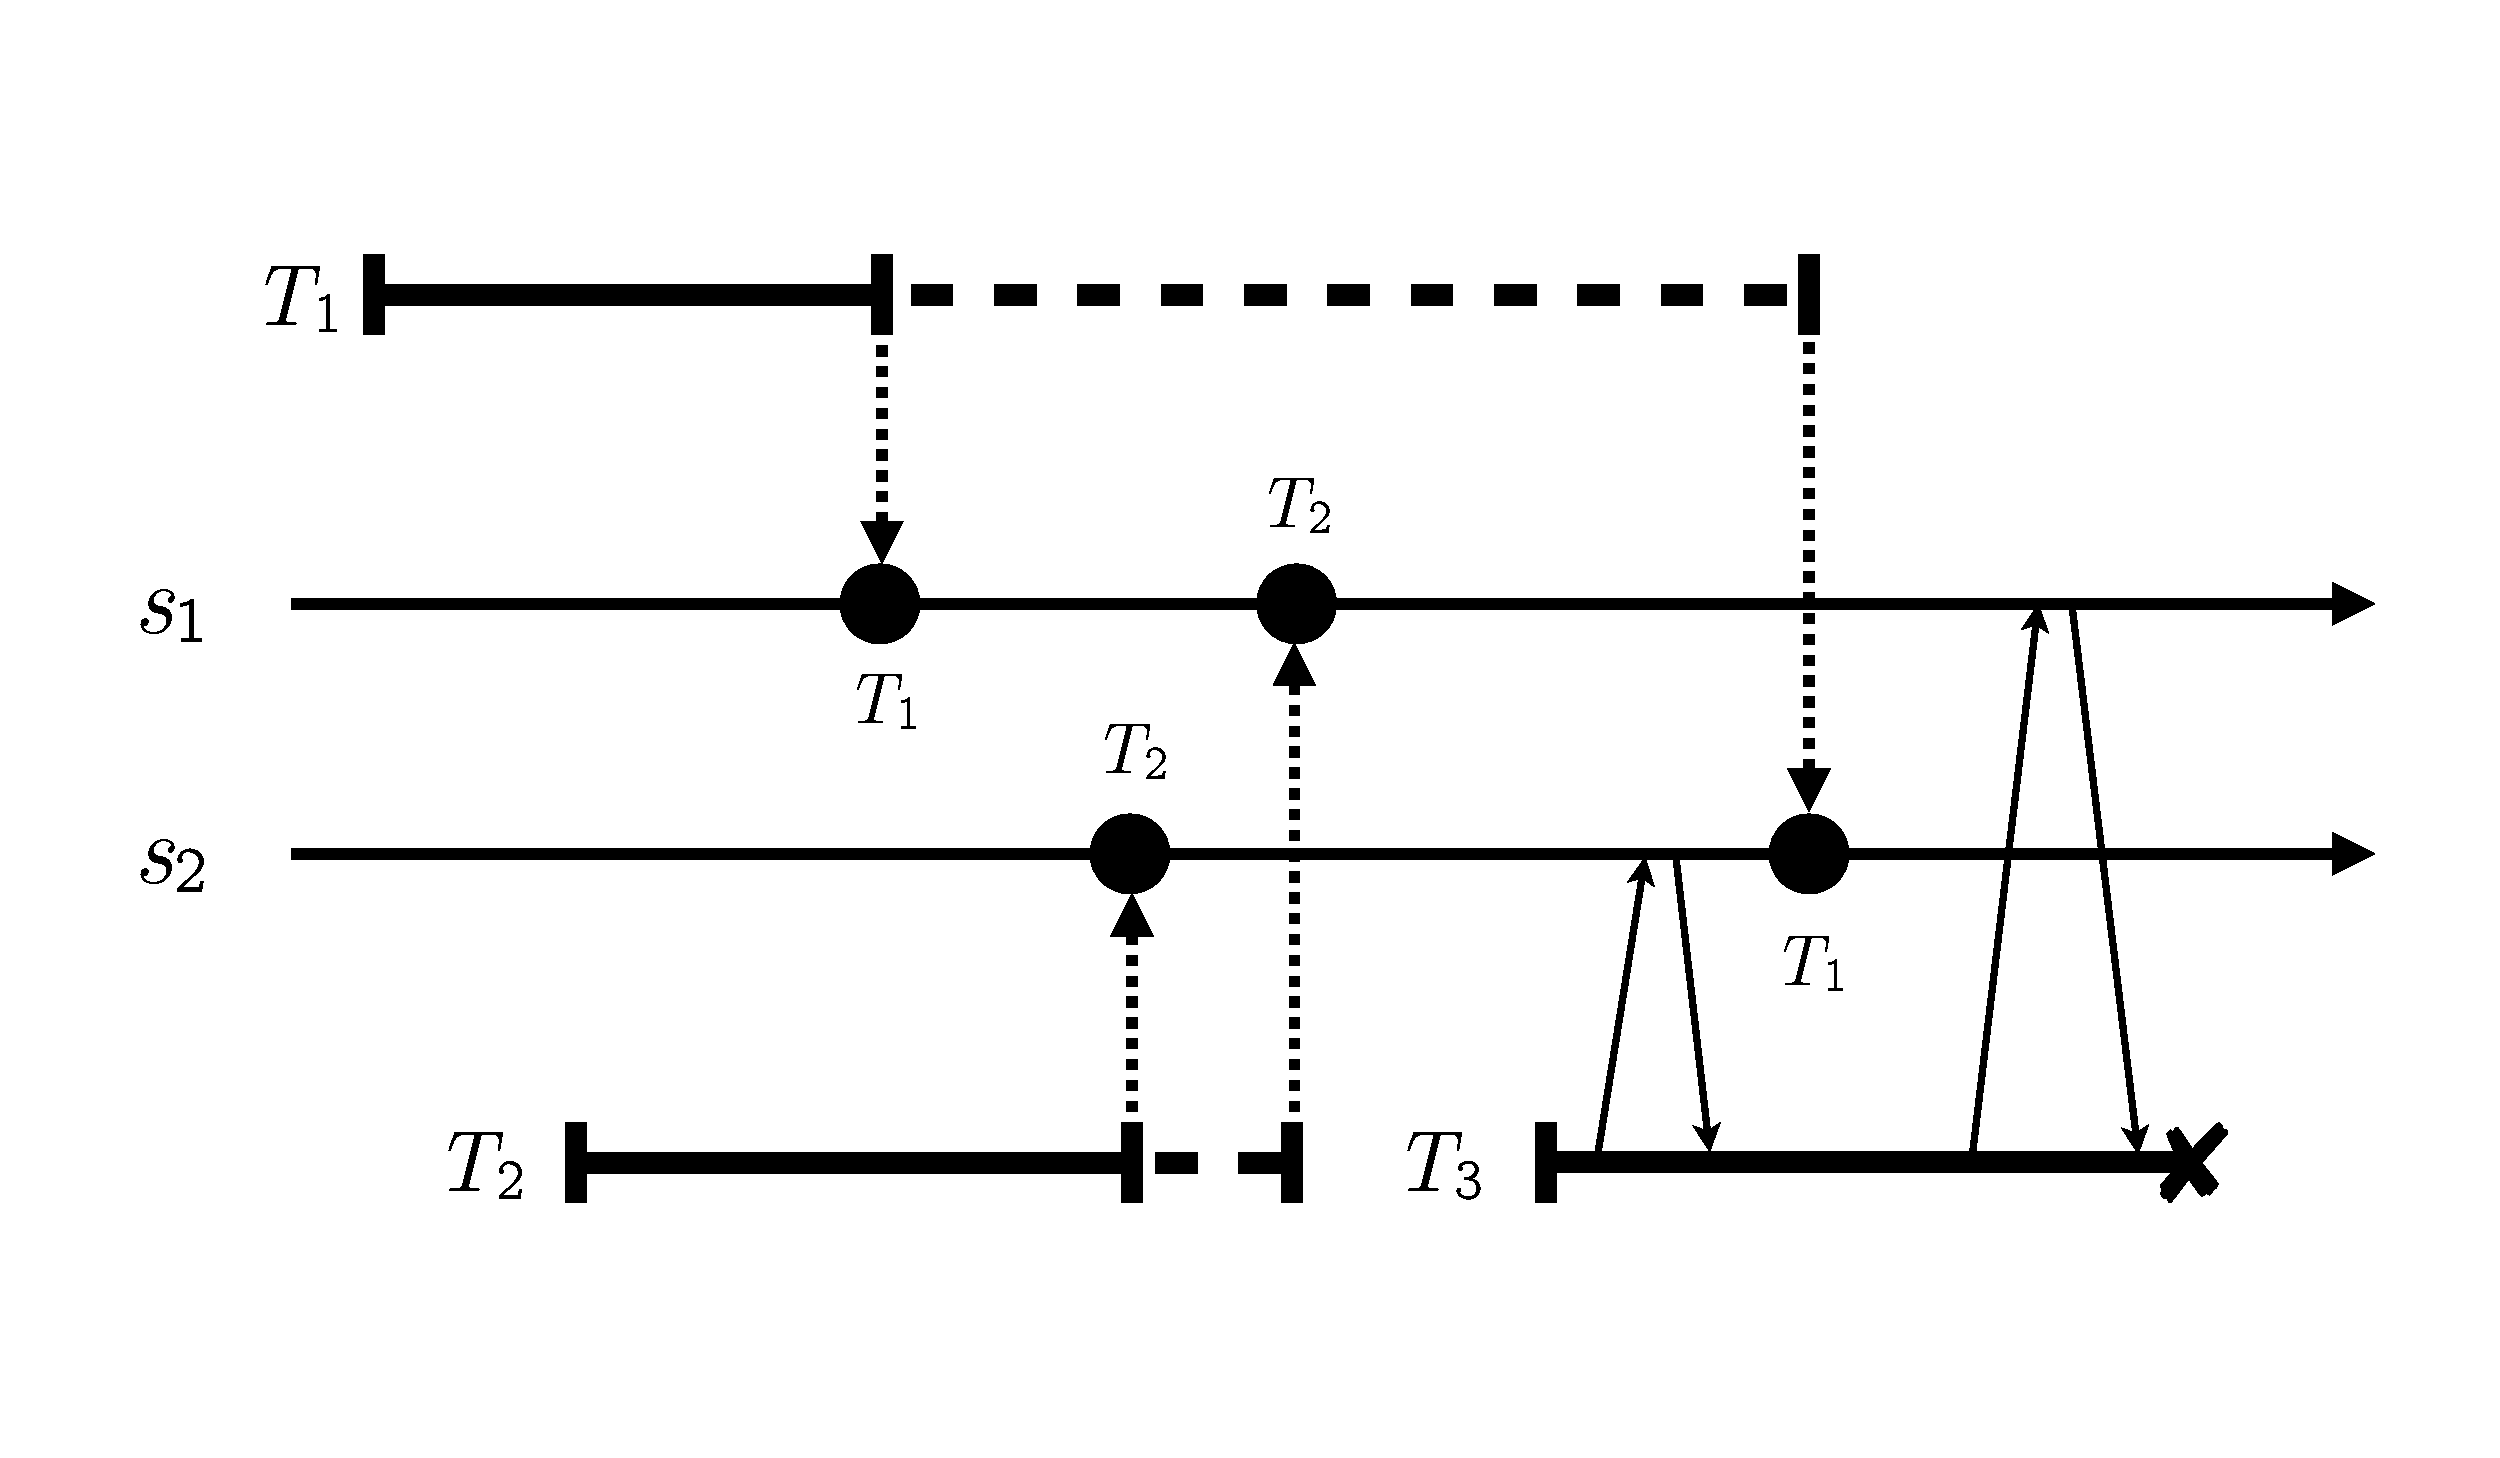
\includegraphics[width=0.6\textwidth]{figures/ch4_abort_execution.pdf}
  \vspace{-0.5cm}
\caption{Example read abort execution. Bold horizontal lines represent executions of transactions over time (left to right), and the big circles represent the commit times of the transactions at different servers. The cross in the execution of $\tx_3$ marks its abort time. }
\label{fig:read_abort}
\end{figure}
